\documentclass[12pt]{article}
\usepackage[commenters={OA,AA,DJM}]{shortex} % adjust initials for comments
\usepackage{authblk}
\usepackage[round]{natbib}
\usepackage[margin=2.5cm]{geometry}
\newcommand{\email}[1]{\href{mailto:#1}{#1}}

% minor adjustments to ShorTeX
\let\argmin\relax\DeclareMathOperator*{\argmin}{argmin}
\let\argmax\relax\DeclareMathOperator*{\argmax}{argmax}
\DeclareMathOperator*{\minimize}{minimize}
\DeclareMathOperator*{\maximize}{maximize}
\DeclareMathOperator{\subjto}{\ \text{subject to}\ }
\renewcommand{\top}{\mathsf{T}}
\renewcommand{\d}{\mathsf{d}}
\newcommand{\cond}{\; \m| \;}

\graphicspath{{../fig/}}
\setlength{\parindent}{0pt}
\setlength{\parskip}{11pt}
\usepackage{enumitem}



% -- Begin document --------------------------------------------------------

\title{\huge Improving the robustness of local $R_t$ estimates during periods of geographical dropout}
\author{Kris V Parag, Daniel J McDonald}
\date{Last revised: \today}

\begin{document}
\maketitle
%\RaggedRight % uncomment to enable ragged right

\section*{Introduction}

\bitem
\item General intro to Rt estimation
\item Discussion of real-time
\item Emphasis on ``local'' methodologies
\item Extension to estimation across many locations simultaneously 
\item Not all locations have the same reporting frequency
\item High-level description of the methods and a ``killer figure'' that shows
what we do.
\eitem


\section*{Results}

This study could combine the algorithm maybe as a small R function that users
can apply to data. There are several questions to investigate that
could complete the paper. 

\begin{figure}
  \centering
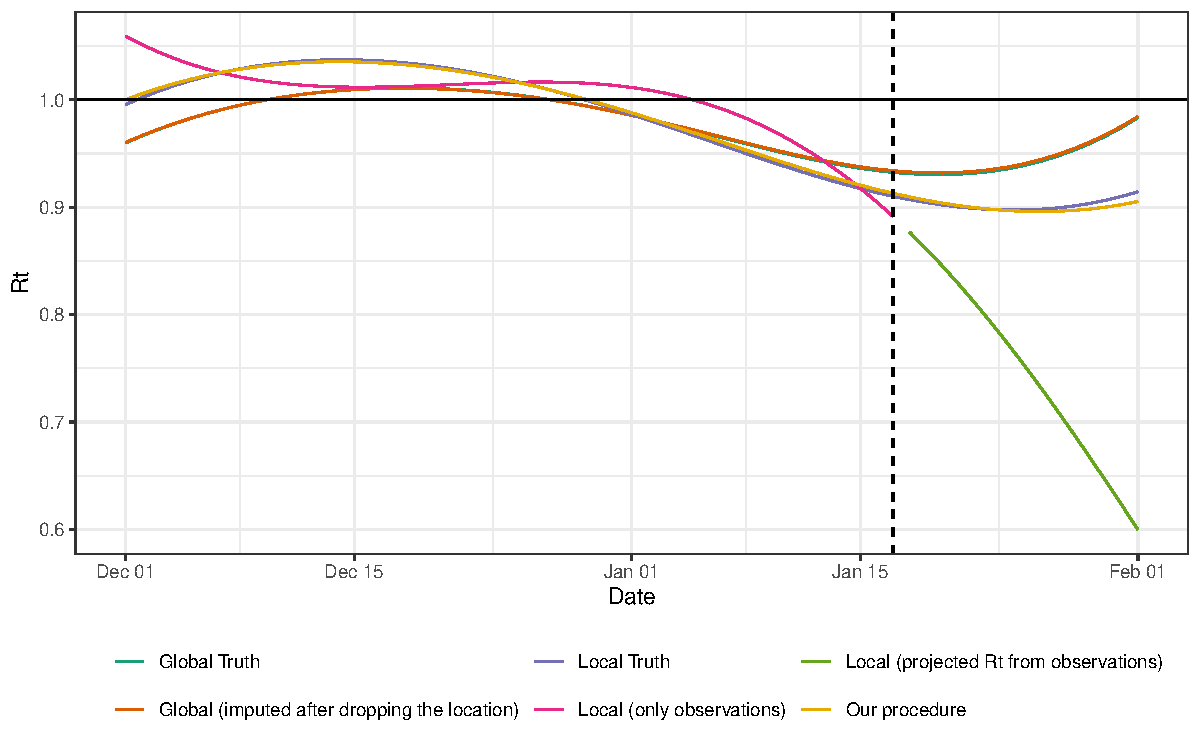
\includegraphics[width=.9\textwidth]{first-fig.pdf}
\caption{A simple motivating example showing Canadian Incidence (nationally) as
well as the results when 15 days of data from British Columbia are artificially
removed.}
\label{fig:prelim1}
\end{figure}

\bitem
\item What is the value of combining local and global information relative to
projecting forward locally? When should this work?
\item How should we define the global scale? Perhaps pick the areas with a
history of having similarly synched epidemics? Nearest neighbours?
\item Given $p$ locations in a region, how many can we tolerate simultaneous
dropout in? What about other patterns? How long (relative to the generation
time) does dropout need to be before there is no chance of correction?
\eitem

Practically, we could combine some more simulated examples using a combination
of the \texttt{rtestim} and \texttt{EpiFilter} code that we already have
developed that can provide insights into when and how global information can
supplement local data scarcity as well as prvide guidelines for when this global
information will not work. This could be about 2 figures. Then about 3 figues
with the more impactful content that uses real examples, perhaps from the CFA
pipeline pr the other data sources we discussed. As baselines we can always
compare to local forecasting and hold out real data to use for validation. 


\section*{Discussion}

Below are some ideas to describe as potential future work.

\bitem
\item Can we inform the additional parameter $\epsilon_h$ in some way to improve
the correction? Does this require other data e.g., mobility?

\item Potential to generalize the methods to more complicated incidence forecasting.
View our simple procedure as a process with 2 modules, a
\texttt{forecaster} and an \texttt{Rtestimator}. Then the meta procedure is

\benum
\item Use \texttt{forecaster} to produce $\{\Lambda_{T+h, \ell}\}$ for $2\leq h
\leq H$. We do this conditional on all available information (incidence at the
location, the region, or some related quantity). 
\item We can supplement these forecasts with auxiliary signals (wastewater,
deaths etc.). Currently, we have a minimal \texttt{forecaster} (uses global $R_t$
and local convolved incidence).
\item Calculate $\hat{I}_{T+h, \ell}$ by taking the first (backward) differences
of $\{\Lambda_{T+h, \ell}\}$.
\item Use \texttt{Rtestimator} once across the pseudo time series to produce
$\{R_{t, \ell}\}_{t=1}^{T+H}$
\eenum

\eitem

\section*{Methods}
\subsection*{Connecting local and global transmission}\label{sec:bayes}

We consider $p\geq 2$ heterogeneous locations (the local scale) that compose a
region of interest (the global scale). We assume that homogeneous mixing is
valid in all locations. We neglect interactions among locations and do not model
geographical movements of infections. As an example of this setup, if our global
scale is at the state level, then our local scale may be at the county level.
Our choice of scales is also determined by the availability of infection data.

We examine two periods of time (usually in units of days). In the first, which
spans $1\leq t \leq T$, we have access to the incidence of new infections (or a
meaningful proxy such as reported cases) in all locations of interest. We denote
this $I_{t, \ell}$ for location $\ell$ at time $t$. The global incidence follows
as the sum over locations and is written as $I_t = \sum_{\ell} I_{t, \ell}$. We
also assume knowledge of the distribution of disease generation times, which is
location independent and defined by probabilities $\omega_i$ such that
$\sum_{i=1}^{\infty}\omega_{i} = 1$.

We can use the renewal transmission model to compute time-varying effective
reproduction numbers at both local and global scales. At a location $\ell$, this
reproduction number is denoted $R_{t, \ell}$ and the corresponding global
reproduction number is $R_{t}$. The renewal models are constructed as in
\eqref{eq: 1} as a Poisson distribution describing intrinsic
stochasticity in generating infections and the $\Lambda$ terms defining the
total infectiousness at a given scale.
\begin{equation}\label{eq: 1}
\begin{aligned}
& I_{t, \ell} \sim \text{Pois} 
\left(R_{t, \ell}\Lambda_{t, \ell}\right) \text{ with } \Lambda_{t, \ell} = \sum_{i=1}^{t-1}
\omega_{i}I_{t-i, \ell} \hspace{0.5cm}\text{(local scale)} \\
& I_t \sim \text{Pois} 
\left(R_t\Lambda_t\right) \text{ with } \Lambda_t = \sum_{i=1}^{t-1}
\omega_{i}I_{t-i} \hspace{0.5cm}\text{(global scale)}
\end{aligned}
\end{equation}

We can replace the Poisson distribution with any noise distribution of interest,
but in this case it is possible to directly connect the transmission scales as
$R_t = \sum_{l=1}^p \Lambda_{t, \ell}R_{t, \ell}\left(\sum_{m=1}^p \Lambda_{t,
m}\right)^{-1}$. Throughout this period up to $T$ we are able to compute
estimates from these models for all locations and globally. These result in
local posterior distributions $\mathbb{P}\left(R_{t, \ell} \cond I_{1,
\ell}^{t}\right)$ and the global posterior $\mathbb{P}\left(R_{t} \cond
\sum_{l=1}^m I_{1, \ell}^{t}\right)$, which are directly obtained from a number
of standard reproduction number estimators. Here, the notation $I_{1, \ell}^{t}$
means the past time series in location $\ell$ from times 1 to $t$.

The second period of interest is from times $T \leq t \leq T+H$. In this period
there is dropout \ie a loss of data in location $\ell$. Consequently, we have no
knowledge of $I_{T, \ell}^{T+h}$ and cannot assess the transmissibility in this
location directly. We consider two options for providing estimates for location
$\ell$ during this period. Across a horizon $1 \leq h \leq H$ we can either:
\benum
\item Project from our last local posterior $\mathbb{P}\left(R_{T, \ell}  \cond
I_{1, \ell}^{T}\right)$ to time $T+h$. This generates the baseline prediction
$\mathbb{P}\left(R_{T+h, \ell}  \cond I_{1, \ell}^{T}\right)$. For a short
enough $h$ this is expected to be reasonable. For large $h$ it simply reproduces
our prior information.
\item Borrow information from the global posteriors (or remaining locations with
data) $\mathbb{P}\left(R_{T+h}  \cond \sum_{m \neq \ell} I_{1, m}^{T+h}\right)$.
This essentially relies on some degree of correlation naturally occurring among
locations due perhaps to similar drivers of spread. We do not assume knowledge
of these correlations.
\item Use a mixture distribution of the above options.
\eenum

\subsection*{Using global transmission to supplement dropout}\label{sec:bayes}

Our main contribution lies in developing a sensible but real-time and
computational simple algorithm to correct estimates in dropout locations. We
propose to use the last local posterior in location $\ell$ as a prior and then
draw information from the global posteriors (which exclude $\ell$) to update
this into the posterior distribution of \eqref{eq: 2}.
\begin{align}
& \mathbb{P}\left(R_{T+1, \ell} \cond I_{1, \ell}^T, \, \sum_{m \neq \ell} 
I_{T+1, m} \right) 
\propto \mathbb{P}\left(R_{T+1, \ell}  \cond \sum_{m \neq \ell}
 I_{T+1, m}\right)\mathbb{P}\left(R_{T+1, \ell}  \cond I_{1, \ell}^{T}\right)
 \label{eq: 2}
\end{align}


This follows due to the conditional independence of the infections in locations.
Later time steps are obtained by iterating this process sequentially (with the
prior reset to the dropout posterior from the last time step). We have not yet
implemented this full version and so test a `deterministic dropout correction'
via the following sequence:

\bitem
\item Because location $\ell$ is unavailable for $t=T+1,\ldots,T+H$, we also
cannot compute $\Lambda_t$ for $t=T+1,\ldots,T+H$. Therefore, we calculate the
{\bf global incidence correction factor}: $\eta = 1 - \Lambda_{\ell,
t}/\Lambda_{t}$. 
\item Compute global $R_t$ by using the adjusted incidence $(I_1,\ldots,I_t, I_{t+1} / \eta, \ldots
I_{t+h} / \eta).$
\item Input $\{R_t\}_{t=1}^{T+H}$, $\{R_{t, \ell}\}_{t=1}^{T}$, $\Lambda_{\ell,t}$.
For $h = 1,\ldots,H$, do
\benum
\item Predict $\hat{I}_{T + h, \ell} = R_{T+h-1}\Lambda_{T+h-1, \ell}$ (expectations from renewal models).
\item Convolve $\Lambda_{T+h, \ell} = \sum_{i=1}^{T+h-1} \omega_{i}\tilde{I}_{T + h
- i}$, where $\tilde{I}_j = I_j \1[j\leq T] + \hat{I}_j \1[j>T]$.
\item Estimate local $\hat{R}_{T+h, \ell} = \epsilon_{h} R_{T+h} \frac{\Lambda_{T+h, \ell}}
{\Lambda_{T+h+1, \ell}}$, with $\epsilon_h$ as a factor we currently set to 1.
\eenum
\item Given $\{\hat{I}_{\ell, t}\}$ and $\{\Lambda_{\ell,t}\}$ for $t=1,\ldots,T+H$, we
recompute the local $R_{t,\ell}$ using both real ($t=1,\ldots,T$) and the
estimated pseudodata ($t=T+1,\ldots,H$).
\eitem





\end{document}

\bibliographystyle{../paper/rss}
\bibliography{../paper/dajmcdon}      
